\chapter{Le tableau périodique~: un premier regard}\label{ch:g9:periodic-table-first-look}

Au mur de presque toutes les salles de chimie est accroché le même
tableau~: 118 cases, chacune portant un symbole et un nombre, rangées en
lignes et en colonnes selon une forme étrange --- de hautes tours sur les
côtés, un creux au milieu, deux lignes détachées en dessous. Quand il fut
dressé pour la première fois, en 1869, il comptait une soixantaine de
cases, dont plusieurs vides. Son auteur eut l'audace de décrire les
éléments qui viendraient un jour combler les trous --- et il avait
raison.

\begin{recall}
Un \omterm{def:g9:inside-the-atom:element}{élément chimique} est l'ensemble des \omterm{def:g7:atoms-and-molecules:atom}{atomes} qui ont le même \omterm{def:g9:inside-the-atom:atomic-number}{numéro
atomique} $Z$, le nombre de \omterm{def:g9:inside-the-atom:proton}{protons} du \omterm{def:g9:inside-the-atom:nucleus}{noyau}
(\cref{ch:g9:inside-the-atom}). Chaque élément a un symbole, une lettre
majuscule parfois suivie d'une minuscule
(\cref{ch:g7:atoms-and-molecules}). Les métaux comme le fer, le zinc et
l'aluminium donnent des \omterm{def:g9:ions:ion}{ions} positifs (\cref{ch:g9:ions}).
\end{recall}

\section{Un tableau des éléments}

\begin{definition}[Tableau périodique]\label{def:g9:periodic-table-first-look:periodic-table}
Le \emph{tableau périodique}\index{tableau periodique@tableau périodique} range tous les
\omterm{def:g9:inside-the-atom:element}{éléments chimiques} par \omterm{def:g9:inside-the-atom:atomic-number}{numéro atomique} croissant, de $Z = 1$ à
$Z = 118$, en lignes disposées de sorte que les éléments aux propriétés
semblables se retrouvent dans la même colonne.
\end{definition}

\begin{definition}[Période et groupe]\label{def:g9:periodic-table-first-look:period}
Une ligne du \omterm{def:g9:periodic-table-first-look:periodic-table}{tableau périodique} est une \emph{période}\index{periode@période}~; il
y en a sept. Une colonne est un \emph{groupe}\index{groupe}~; il y en a
dix-huit, numérotés de 1 à 18 de gauche à droite. Les deux lignes
imprimées sous le tableau appartiennent aux périodes 6 et 7~; on ne les
met à part que pour garder un tableau étroit.
\end{definition}

\begin{omfigure}
\omperiodictable[colour=metals, legend=true, cell=0.86cm]

{\small Le \omterm{def:g9:periodic-table-first-look:periodic-table}{tableau périodique}. Chaque case donne le \omterm{def:g9:inside-the-atom:atomic-number}{numéro atomique} et
le symbole. Couleurs~: les métaux, les métalloïdes (éléments
intermédiaires entre métaux et non-métaux) et les non-métaux, selon la
classification habituelle.}
\end{omfigure}

\begin{method}[Lire le tableau périodique]\label{met:g9:periodic-table-first-look:read}
Pour situer un élément~:
\begin{enumerate}
  \item trouver sa case grâce à son symbole ou à son \omterm{def:g9:inside-the-atom:atomic-number}{numéro atomique}~;
  \item sa ligne donne sa \omterm{def:g9:periodic-table-first-look:period}{période}, sa colonne son groupe~;
  \item sa couleur indique s'il s'agit d'un \omterm{def:g9:periodic-table-first-look:metal}{métal} ou d'un \omterm{def:g9:periodic-table-first-look:metal}{non-métal}.
\end{enumerate}
Le sodium, \ce{Na}, $Z = 11$~: \omterm{def:g9:periodic-table-first-look:period}{période} 3, \omterm{def:g9:periodic-table-first-look:period}{groupe} 1, un \omterm{def:g9:periodic-table-first-look:metal}{métal}. Le chlore,
\ce{Cl}, $Z = 17$~: \omterm{def:g9:periodic-table-first-look:period}{période} 3, \omterm{def:g9:periodic-table-first-look:period}{groupe} 17, un \omterm{def:g9:periodic-table-first-look:metal}{non-métal}.
\end{method}

\section{Métaux et non-métaux}

\begin{definition}[Métal et non-métal]\label{def:g9:periodic-table-first-look:metal}
Un \emph{métal}\index{metal@métal} est un élément qui, à l'état de \omterm{def:g6:pure-substances-and-mixtures:pure-substance}{corps pur},
est brillant quand on vient de le couper, conduit bien l'électricité et
la chaleur, peut être plié ou mis en forme au marteau, et forme des \omterm{def:g9:ions:ion}{ions}
positifs. Un \emph{non-métal}\index{non-metal@non-métal} n'a pas ces propriétés~:
beaucoup sont des gaz (le dioxygène, le diazote, le dichlore), ceux qui
sont solides sont ternes et cassants (le soufre, le carbone sous forme
de charbon), et ils tendent à former des \omterm{def:g9:ions:ion}{ions} négatifs ou à mettre en
commun des \omterm{def:g9:inside-the-atom:nucleus}{électrons} dans des \omterm{def:g7:atoms-and-molecules:molecule}{molécules}.
\end{definition}

\begin{proposition}[Où ils se trouvent]\label{prop:g9:periodic-table-first-look:where}
Environ quatre éléments sur cinq sont des métaux~; ils occupent la
gauche et le centre du tableau. Les non-métaux se trouvent en haut à
droite, avec l'hydrogène seul en haut à gauche. Le long de la frontière
entre les deux, quelques éléments --- le bore, le silicium, le
germanium, l'arsenic, l'antimoine, le tellure --- ont des propriétés
intermédiaires~: ce sont les métalloïdes.
\end{proposition}

\section{Des colonnes qui se ressemblent}

\begin{proposition}[Les éléments d'un groupe se comportent de façon semblable]\label{prop:g9:periodic-table-first-look:alike}
Les éléments d'un même groupe réagissent de façon semblable et forment
des composés semblables. Le lithium, le sodium et le potassium, en haut
du \omterm{def:g9:periodic-table-first-look:period}{groupe} 1, sont des métaux mous qui réagissent avec l'eau en dégageant
du dihydrogène~; la réaction est plus violente quand on descend dans le
groupe. Le fluor, le chlore, le brome et l'iode, du \omterm{def:g9:periodic-table-first-look:period}{groupe} 17, sont des
non-métaux colorés qui réagissent avec les métaux pour former des sels.
L'hélium, le néon, l'argon et les autres éléments du \omterm{def:g9:periodic-table-first-look:period}{groupe} 18 ne
réagissent presque avec rien.
\end{proposition}

\begin{inthelab}[Le lithium, le sodium et le potassium dans l'eau]
Derrière un écran de protection, l'enseignant laisse tomber un morceau
de lithium de la taille d'un grain de riz dans une grande cuvette d'eau~:
il pétille doucement. Un morceau de sodium de même taille file à la
surface en fondant en une bille argentée. Le potassium s'enflamme
aussitôt avec une flamme lilas. Tous trois dégagent du dihydrogène et
laissent une \omterm{def:g9:acids-bases-ph:acidic}{solution basique}.
\end{inthelab}

\begin{safety}{\ghs[0.82cm]{GHS02}\ghs[0.82cm]{GHS05}}
% ledger: ghs:Na
Le sodium, au contact de l'eau, libère des gaz inflammables qui peuvent
s'enflammer spontanément (GHS02)~; il provoque de graves brûlures
(GHS05). On le conserve sous huile, et seul l'enseignant le manipule,
avec une pince, en tout petits morceaux.
\end{safety}

\section{L'idée de Mendeleïev}

\begin{history}[Les cases vides de Mendeleïev, 1869--1886]
En 1869, Dmitri Mendeleïev rangea les éléments alors connus par masse
atomique croissante --- la masse de leurs \omterm{def:g7:atoms-and-molecules:atom}{atomes} comparée à celle de
l'hydrogène --- et plaça côte à côte ceux qui avaient des propriétés
semblables. Là où la régularité l'exigeait, il laissa des cases vides
pour des éléments que personne n'avait encore trouvés, et en 1871 il
décrivit leurs propriétés~: sous le silicium, un «~éka-silicium~» dont
la masse atomique serait d'environ 72. En 1886, le chimiste Clemens
Winkler découvrit le germanium dans un \omterm{def:g5:raw-materials-and-recycling:raw-material}{minerai} d'argent, mesura sa masse
atomique, 72.3, et montra qu'il s'agissait de l'élément manquant. Le
gallium (1875) et le scandium (1879) vinrent aussi combler des cases
laissées vides par Mendeleïev.
\end{history}

\begin{omfigure}
\begin{minipage}[b]{0.32\linewidth}\centering
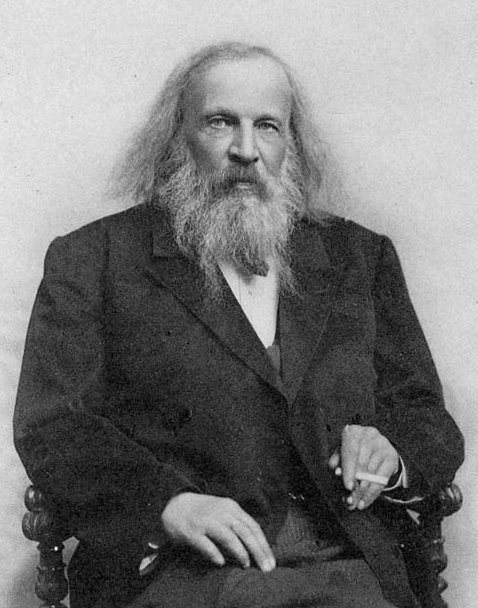
\includegraphics[width=\linewidth]{images/book1/mendeleev.jpg}

{\small Dmitri Mendeleïev (1834--1907).}
\end{minipage}\hfill
\begin{minipage}[b]{0.6\linewidth}\centering
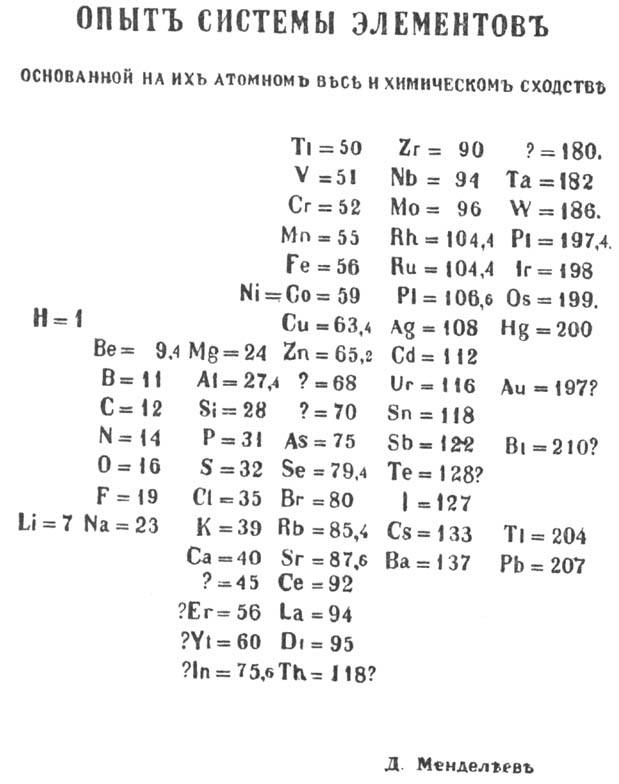
\includegraphics[width=0.85\linewidth]{images/book1/mendeleev-1869.jpg}

{\small Le tableau de Mendeleïev de 1869, en russe. À côté de Si $= 28$
et Al $= 27.4$, les cases «~? $= 70$~» et «~? $= 68$~» attendent le
germanium et le gallium.}
\end{minipage}
\end{omfigure}

\begin{remark}[L'ordre des numéros atomiques]\label{rem:g9:periodic-table-first-look:order}
Mendeleïev rangeait les éléments par masse atomique, et dut intervertir
quelques paires, comme le tellure et l'iode, pour garder les familles
ensemble. Aujourd'hui, le tableau est rangé par \omterm{def:g9:inside-the-atom:atomic-number}{numéro atomique}, une
notion découverte plus tard, et ces interversions ne sont plus
nécessaires.
\end{remark}

\section{Exercices}

\begin{exercise}[$\star$]\label{exo:g9:periodic-table-first-look:1}
Dans quel ordre les éléments sont-ils placés dans le \omterm{def:g9:periodic-table-first-look:periodic-table}{tableau
périodique}~?
\end{exercise}

\begin{exercise}[$\star$]\label{exo:g9:periodic-table-first-look:2}
Donne la \omterm{def:g9:periodic-table-first-look:period}{période} et le groupe~: du carbone ($Z = 6$), du magnésium
($Z = 12$), de l'argon ($Z = 18$).
\end{exercise}

\begin{exercise}[$\star$]\label{exo:g9:periodic-table-first-look:3}
\omterm{def:g9:periodic-table-first-look:metal}{Métal} ou \omterm{def:g9:periodic-table-first-look:metal}{non-métal}~: le fer, le soufre, le cuivre, l'oxygène,
l'aluminium, le chlore~?
\end{exercise}

\begin{exercise}[$\star$]\label{exo:g9:periodic-table-first-look:4}
Quel élément se trouve juste sous le sodium dans le tableau~? Juste sous
le chlore~?
\end{exercise}

\begin{exercise}[$\star\star$]\label{exo:g9:periodic-table-first-look:5}
À l'aide du tableau, nomme l'élément de la \omterm{def:g9:periodic-table-first-look:period}{période} 4 et du \omterm{def:g9:periodic-table-first-look:period}{groupe} 2, et
l'élément de la \omterm{def:g9:periodic-table-first-look:period}{période} 2 et du \omterm{def:g9:periodic-table-first-look:period}{groupe} 15.
\end{exercise}

\begin{exercise}[$\star\star$]\label{exo:g9:periodic-table-first-look:6}
Pourquoi peut-on s'attendre à ce que le potassium réagisse avec l'eau,
comme le sodium~?
\end{exercise}

\begin{exercise}[$\star\star$]\label{exo:g9:periodic-table-first-look:7}
Un élément brillant conduit l'électricité et forme l'\omterm{def:g9:ions:ion}{ion} \ce{X^{2+}}.
Est-ce un \omterm{def:g9:periodic-table-first-look:metal}{métal} ou un \omterm{def:g9:periodic-table-first-look:metal}{non-métal}~? Explique.
\end{exercise}

\begin{exercise}[$\star\star$]\label{exo:g9:periodic-table-first-look:8}
Pourquoi Mendeleïev a-t-il laissé des cases vides dans son tableau~?
Pourquoi était-ce une force de son tableau plutôt qu'une faiblesse~?
\end{exercise}

\begin{exercise}[$\star\star$]\label{exo:g9:periodic-table-first-look:9}
Regarde le tableau de Mendeleïev de 1869. Quelles masses atomiques
donnait-il au carbone et à l'oxygène~? Quelles cases vides, marquées
d'un point d'interrogation, apparaissent à côté de l'aluminium et du
silicium~?
\end{exercise}

\begin{exercise}[$\star\star$]\label{exo:g9:periodic-table-first-look:10}
Combien y a-t-il d'éléments dans la \omterm{def:g9:periodic-table-first-look:period}{période} 2~? Dans la \omterm{def:g9:periodic-table-first-look:period}{période} 4~?
\end{exercise}

\begin{exercise}[$\star\star\star$]\label{exo:g9:periodic-table-first-look:11}
L'hélium, le néon et l'argon ne réagissent presque avec rien. Dans quel
groupe sont-ils~? À quoi pourraient-ils servir, compte tenu de cette
propriété~?
\end{exercise}

\begin{exercise}[$\star\star\star$]\label{exo:g9:periodic-table-first-look:12}
Le gallium, sous l'aluminium, a été découvert en 1875. Mendeleïev lui
avait prédit une masse atomique proche de la moyenne de celles de ses
voisins l'aluminium (27.0) et l'indium (114.8). Calcule cette moyenne.
(Gallium~: 69.7.)
\end{exercise}

\section{Problème~: la case vide de Mendeleïev}

\begin{problem}[{Problème du week-end --- prévoir la masse atomique d'un
élément manquant à partir de ses quatre voisins}]
\label{pb:g9:periodic-table-first-look:1}
% ledger: aw:Si, aw:Sn, aw:Ga, aw:As, aw:Ge, mend:eka-si-aw, ge:winkler-aw
En 1871, Mendeleïev prédit les propriétés de l'éka-silicium, l'élément
manquant sous le silicium. L'une de ses idées était que les propriétés
d'un élément se situent entre celles de ses voisins du dessus et du
dessous, de gauche et de droite. Les masses atomiques actuelles des
quatre voisins de la case vide sont~: silicium 28.1 (au-dessus), étain
118.7 (au-dessous), gallium 69.7 (à gauche), arsenic 74.9 (à droite).

\medskip
\noindent\textbf{Partie I --- La case vide.}
\begin{enumerate}
  \item À l'aide du \omterm{def:g9:periodic-table-first-look:periodic-table}{tableau périodique} de ce chapitre, trouve le \omterm{def:g9:inside-the-atom:atomic-number}{numéro
        atomique}, la \omterm{def:g9:periodic-table-first-look:period}{période} et le groupe du germanium, l'élément qui
        comble la case vide.
  \item Quel élément est au-dessus de lui, lequel au-dessous, lequel à
        sa gauche, lequel à sa droite~?
  \item Le germanium est-il un \omterm{def:g9:periodic-table-first-look:metal}{métal}, un \omterm{def:g9:periodic-table-first-look:metal}{non-métal} ou un métalloïde~?
  \item Pourquoi Mendeleïev s'attendait-il à ce que l'élément manquant
        ressemble au silicium~?
\end{enumerate}

\medskip
\noindent\textbf{Partie II --- Les moyennes.}
\begin{enumerate}[resume]
  \item Calcule la moyenne des masses atomiques des éléments situés
        au-dessus et au-dessous de la case vide.
  \item Calcule la moyenne des masses atomiques des éléments situés à
        gauche et à droite.
  \item Laquelle des deux moyennes est la plus proche de la vraie masse
        atomique du germanium, 72.6~? Pourquoi pourrait-il en être
        ainsi~?
  \item Dans son tableau de 1869, Mendeleïev avait écrit «~? $= 70$~»
        pour cette case. De combien se trompait-il~?
\end{enumerate}

\medskip
\noindent\textbf{Partie III --- La prédiction.}
\begin{enumerate}[resume]
  \item Calcule la moyenne des quatre voisins, au dixième près.
  \item En 1871, Mendeleïev prédisait 72~; en 1886, Winkler mesura 72.3.
        Compare avec ta moyenne.
  \item Pourquoi la découverte du germanium a-t-elle convaincu beaucoup
        de chimistes que le tableau de Mendeleïev était juste~?
  \item Formule ta prédiction~: la masse atomique de l'éka-silicium
        d'après la moyenne de ses quatre voisins.
\end{enumerate}
\end{problem}
